%Master File:lectures.tex


\lesson{Entropy}
\vspace{-1cm}
\begin{center}
  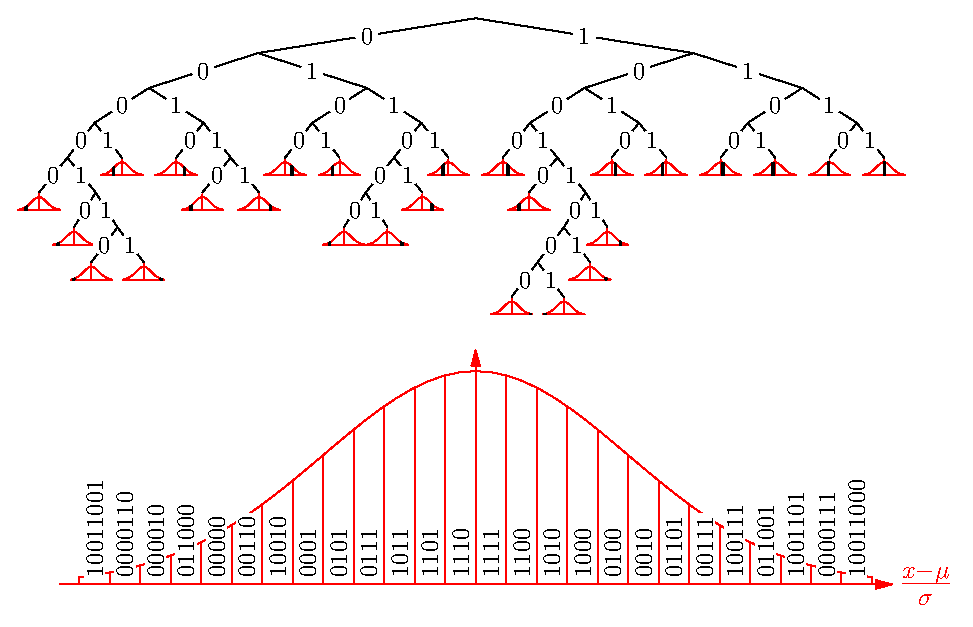
\includegraphics[height=10cm]{huffman}
\end{center}
\keywords{Entropy, Coding, Maximum Entropy}
%%%%%%%%%%%%%%%%%%%%%%% Next Slide %%%%%%%%%%%%%%%%%%%%%%%
\renewcommand{\Outline}{%
\begin{slide}
\section[1]{Outline}

\begin{minipage}{10cm}\raggedright
  \begin{enumerate}\squeeze
    \outlineitem{Measuring Uncertainty}{uncertainty}
    \outlineitem{Code Length}{code}
    \outlineitem{Maximum Entropy}{maxentropy}
  \end{enumerate}
\end{minipage}\hfill
\begin{minipage}{12cm}
  \includegraphics[width=12cm]{maxent}
\end{minipage}
\end{slide}
\addtocounter{outlineitem}{1}
}

\newcommand{\bits}{\,\mathrm{bits}}
\setcounter{outlineitem}{1}
\Outline % Motivation
\toptarget{firstoutline}
%%%%%%%%%%%%%%%%%%%%%%% Next Slide %%%%%%%%%%%%%%%%%%%%%%%

\begin{slide}
\section{Measuring Uncertainty}
  
\begin{PauseHighLight}
  \begin{itemize}
  \item What is more uncertain tossing a coin three times or throwing
    a dice\pause
  \item The answer depends on whether you care about the order of the
    coin tosses\pause
  \item But, how do we answer such a question?\pause
  \item Let $X$ be a random variable denoting the possible outcomes\pause
  \item Interestingly, Shannon entropy give a precise answer
    \begin{align*}
      H_X = -\sum_{x\in\mathcal{X}} \Prob{X=x}\, \logtwo{\Prob{X=x}}\pause
    \end{align*}
  \end{itemize}
\end{PauseHighLight}

\end{slide}

%%%%%%%%%%%%%%%%%%%%%%% Next Slide %%%%%%%%%%%%%%%%%%%%%%%

\begin{slide}
\section{Let's Calculate}

\begin{PauseHighLight}
  \begin{itemize}
  \item For an honest dice $D \in\{1,2,3,4,5,6\}$ and $\Prob{D=i} = 1/6$
    so
    \begin{align*}
      H_D = - \sum_{i=1}^6 \frac{1}{6} \logtwo{ \frac{1}{6}} = - \logtwo{
      \frac{1}{6}} = \log_2(6) \approx 2.584 \bits\pause
    \end{align*}
  \item For an honest coin where we care about the order so $C \in
    \{000,001,\ldots, 111\}$ the $\Prob{C=i} = \frac{1}{8}$ and
    \begin{align*}
      H_C = - \sum_{i=0}^7 \frac{1}{8} \logtwo{ \frac{1}{8}} = - \logtwo{
      \frac{1}{8}} = \log_2(8) = 3 \bits\pause
    \end{align*}
  \item This clearly makes sense: there are more possible outcomes; all
    equally likely\pause
  \end{itemize}
\end{PauseHighLight}


\end{slide}

%%%%%%%%%%%%%%%%%%%%%%% Next Slide %%%%%%%%%%%%%%%%%%%%%%%

\begin{slide}
\section{Unordered Coin Toss}

\begin{PauseHighLight}
  \begin{itemize}
  \item What if we don't care about the order of the out-come then
    $\Prob{HHH}=\Prob{TTT}=1/8$, $\Prob{HHT}=\Prob{HTT}=3/8$ so
    \begin{align*}
      H_U = -\frac{1}{4} \logtwo{\frac{1}{8}} - \frac{3}{4}
      \logtwo{\frac{3}{8}}\approx 1.811 \bits\pause
    \end{align*}
  \item This seems reasonable, although it is not obvious how you
    would determine this without using entropy\pause
  \item But why Shannon entropy?\pauseb
  \end{itemize}
\end{PauseHighLight}

\end{slide}

%%%%%%%%%%%%%%%%%%%%%%% Next Slide %%%%%%%%%%%%%%%%%%%%%%%

\begin{slide}
\section[-2]{Additive Entropy}

\begin{PauseHighLight}
  \begin{itemize}
  \item If $H_X$ and $H_Y$ is the uncertainty of two independent random
    variable $X$ and $Y$, what  is the uncertainty of the combined
    event $(X,Y)$?
    \begin{align*}
      H_{(X,Y)}
      &= -\sum_{X,Y} \Prob{X,Y} \, \logtwo{\Prob{X, Y}}\pause\\
      &= -\sum_{X,Y} \Prob{X}\Prob{Y} \, \logtwo{\Prob{X} \Prob{Y}}\pause\\
      &= -\sum_{X,Y} \Prob{X}\Prob{Y} \,\left(  \strut\logtwo{\Prob{X}}+
        \logtwo{\Prob{Y}} \right)\pause\\
      &= -\sum_X \Prob{X}\,\logtwo{\Prob{X}} - \sum_Y
        \Prob{Y}\,\logtwo{Y}\pause
        = H_X + H_Y\pause
    \end{align*}
  \item Shannon's entropy is one of the few functions that satisfy
    this condition\pause
  \end{itemize}
\end{PauseHighLight}

\end{slide}


%%%%%%%%%%%%%%%%%%%%%%% Next Slide %%%%%%%%%%%%%%%%%%%%%%%
\Outline % Code Length
%%%%%%%%%%%%%%%%%%%%%%% Next Slide %%%%%%%%%%%%%%%%%%%%%%%

\begin{slide}
\section[-2]{Why Measure Entropy in Bits}
  
\begin{PauseHighLight}
  \begin{itemize}
  \item Suppose we had to communicate a message with $2^n$ equally
    likely outputs (e.g. the result of $n$-coin tosses)\pause
  \item We can do this with a binary string with $n$ bits
    (011..0)\pause
  \item If there were 5 possible outcomes I could do this with 3 bits,
    but waste 3/8 of the message\pause
  \item However if we have a batch of 3 independent messages each with 5
    outcomes then there are 125 possible outcomes\pause.  We could communicate
    this with 8 bits.  This would waste 3/128 of the message\pauseb
  \item By batching together enough messages  with $N$ outcomes then
    we asymptotically  need just $\log_2(N)$ bits\pause
  \end{itemize}
\end{PauseHighLight}

\end{slide}

%%%%%%%%%%%%%%%%%%%%%%% Next Slide %%%%%%%%%%%%%%%%%%%%%%%

\begin{slide}
\section[-2]{Different Probabilities}

\pb
  \begin{itemize}
  \item We ``showed'' that if we had $N$ events, $X_i$, each with
    probability, $\Prob{X_i} = 1/N$, we can code the outcomes with a
    message of length $-\logtwo{\Prob{X_i}}\pause=\logtwo{N}$\pauseb
  \item With a shorter message we would not be able to distinguish all
    possible outcomes from the message\pauseh
  \item What happens if some of outcomes occur with a different probability\pauseh \pauselevel{=1, =2, =3}
    \begin{center}
      \multipdf[width=0.9\linewidth]{diceEntropy}\pause
    \end{center}
  \end{itemize}

\end{slide}

%%%%%%%%%%%%%%%%%%%%%%% Next Slide %%%%%%%%%%%%%%%%%%%%%%%

\begin{slide}
\section[-1]{Shannon's Entropy}

\begin{PauseHighLight}
  \begin{itemize}
  \item If the probabilities are not equal to $2^{-n}$ we can
    still find a code with a length very close to $-\logtwo{\Prob{X}}$
    per message by transmitting a large number of messages\pause
  \item The length of the message measures the amount of
    \emph{surprise} on receiving the message\pause
  \item Shannon's entropy is the expected length of the message to
    communicate a random variable $X$
    \begin{align*}
      H_X = \av[X]{-\logtwo{\Prob{X}}}
      = - \sum_{x\in\mathcal{X}} \Prob{X=x}\, \logtwo{\Prob{X=x}}\pause
    \end{align*}
  \item The expected length is a measure of the uncertainty\pause{} (how much
    information on average we need to convey the outcome)\pauseb
  \end{itemize}
\end{PauseHighLight}
  

\end{slide}

%%%%%%%%%%%%%%%%%%%%%%% Next Slide %%%%%%%%%%%%%%%%%%%%%%%

\begin{slide}
\section[-1]{Real Codes}

\begin{PauseHighLight}
  \begin{itemize}
  \item Those of you with some computer science background will
    realise that we can't actually use different length strings in a
    code without paying some price\pause
  \item We won't know where a code word ends so we can't decode the
    message\pause
  \item An optimal solution is to use Huffman encoding where we
    associate the leaf of a tree with each code word\pause
  \item Using the tree we can decode any message constructed using the
    tree\pause
  \item There is a greedy algorithm for constructing the optimal
    tree\pause
  \end{itemize}
\end{PauseHighLight}

\end{slide}

%%%%%%%%%%%%%%%%%%%%%%% Next Slide %%%%%%%%%%%%%%%%%%%%%%%

\begin{slide}
\section[-2]{Coding Normals}

\begin{center}
  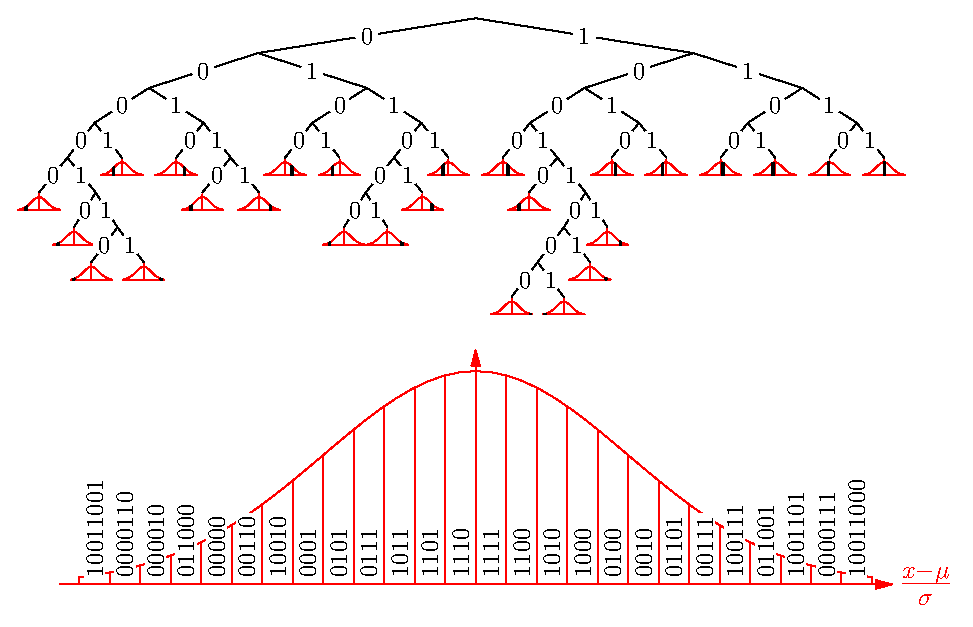
\includegraphics[width=\linewidth]{huffman}
\end{center}
\end{slide}

%%%%%%%%%%%%%%%%%%%%%%% Next Slide %%%%%%%%%%%%%%%%%%%%%%%

\begin{slide}
\section{Coding Normals to Accuracy $\Delta x$}

\pb \pause \pauselevel{=1}
\begin{center}
  \multipdf[width=0.9\linewidth]{huffman2}\pause
\end{center}
\end{slide}


%%%%%%%%%%%%%%%%%%%%%%% Next Slide %%%%%%%%%%%%%%%%%%%%%%%

\begin{slide}
\section{bits and nats}

\begin{PauseHighLight}
  \begin{itemize}
  \item We have measured entropy in \emph{bits} using
    \begin{align*}
      H_X = - \sum_{x\in\mathcal{X}} \Prob{X=x} \, \logtwo{\strut \Prob{X=x}}\pause
    \end{align*}
  \item Sometimes it is easier to use natural logarithms
    \begin{align*}
      H_X = - \sum_{x\in\mathcal{X}} \Prob{X=x} \, \ln\!\bra{\strut \Prob{X=x}}\pause
    \end{align*}
  \item In this case the entropy is measured in \emph{nats} with 1 nat
    equal to $\log_2(\mathrm{e})$ bits\pause
  \item This is often easier when we want to do calculus on entropy\pause
  \end{itemize}
\end{PauseHighLight}

\end{slide}


%%%%%%%%%%%%%%%%%%%%%%% Next Slide %%%%%%%%%%%%%%%%%%%%%%%
\Outline % Maximum Entropy
%%%%%%%%%%%%%%%%%%%%%%% Next Slide %%%%%%%%%%%%%%%%%%%%%%%

\begin{slide}
\section[-2]{Number of States}

\begin{PauseHighLight}
  \begin{itemize}
  \item Suppose I have $N$ balls I them put in $K$ boxes with coordinates
    $x_i$ such that the mean is $\mu$ and variance is $\sigma^2$\pause
    \begin{center}
      \includegraphics[width=0.6\linewidth]{maxent}
    \end{center}
    \begin{align*}
      \Prob{\bm{n}} &\propto \frac{N!}{n_1!\,n_2!\cdots n_K!}
                      \pred{ \sum_i \frac{n_i}{N} x_i = \mu }
                      \pred{ \sum_i \frac{n_i}{N} (x_i-\mu)^2 = \sigma^2 } \pause
    \end{align*}
  \end{itemize}
\end{PauseHighLight}

\end{slide}

%%%%%%%%%%%%%%%%%%%%%%% Next Slide %%%%%%%%%%%%%%%%%%%%%%%

\begin{slide}
\section[0]{Stirling's Approximation}

\begin{rightImage}[0.2]{stirling}
  \begin{PauseHighLight}
  \small
  \begin{itemize}
  \item We can approximate the factorial $n!$ using \emph{Stirling's
      approximation}
    \begin{align*}
      n! &\approx \sqrt{2\,\pi\,n}\, n^n\,\e{-n} \\
      \log(n!) &= n \log(n) - n + \frac{1}{2}\log(2\,\pi\,n)\pause
    \end{align*}
  \item Using this in our formula for $\Prob{\bm{n}}$ we have
    \begin{align*}
      \Prob{\bm{n}} \approx C \, \E{- N \sum_i \frac{n_i}{N} \logg{\frac{n_i}{N}} }
      \prod_{l=1}^3 \pred{ \sum_i \frac{n_i}{N} f_l(x_i) = v_l }\pauseh
    \end{align*}
    where $(f_1(x_i), v_l) = \left\{\strut (1,1), (x_i, \mu),
      ((x_i-\mu)^2, \sigma^2) \right\}$\pause
  \end{itemize}
  \end{PauseHighLight}
\end{rightImage}
\end{slide}

%%%%%%%%%%%%%%%%%%%%%%% Next Slide %%%%%%%%%%%%%%%%%%%%%%%

\begin{slide}
\section[-2]{Number of States and Entropy}
  
\begin{PauseHighLight}
  \begin{itemize}
  \item Let $p(x_i) = n_i/N$ be the proportion of balls in bin $i$ then
    \begin{align*}
      \Prob{\bm{n}} \approx C \e{N\,H_X} \,  \prod_{l=1}^3 \pred{ \sum_i \frac{n_i}{N} f_l(x_i) = v_l }
    \end{align*}
    where
    \begin{align*}
      H_X = -\sum_{i} p(x_i)\, \logg{p(x_i)}\pause
    \end{align*}
  \item That is, the ``entropy'' can be seen as a measure of the
    logarithm of the number of configurations\pause
  \item When the number of balls, $N\rightarrow\infty$ the
    overwhelmingly likely configurations is the one that maximises the
    entropy subject to the observed mean and variance\pause
  \end{itemize}
\end{PauseHighLight}

\end{slide}

%%%%%%%%%%%%%%%%%%%%%%% Next Slide %%%%%%%%%%%%%%%%%%%%%%%

\begin{slide}
\section{Maximum Entropy Method}

\begin{PauseHighLight}
  \begin{itemize}
  \item When we are trying to infer a distribution given some
    observations then we can maximise the entropy subject to
    constraints\pause---the entropy acts as a prior\pauseb
  \item This is known as the \emph{maximum entropy method}\pause
  \item We can rationalise this as this is by far the most likely set
    of configurations consistent with the observations\pause
  \item Alternatively we can see this as maximising our uncertainty
    given what we know\pause---being as unbiased as possible\pauseb
  \item It only gives a good approximation if all possibilities are
    equally likely\pause
  \end{itemize}
\end{PauseHighLight}

\end{slide}

%%%%%%%%%%%%%%%%%%%%%%% Next Slide %%%%%%%%%%%%%%%%%%%%%%%

\begin{slide}
\section[-2]{Knowing the Mean and Variance}

\begin{PauseHighLight}\small
  \begin{itemize}
  \item Consider a continuous random variable, $X$, with a known mean and
    second moment
    \vspace*{-2cm}
    
    \begin{align*}
      \av{X} &= \mu, & \av{X^2} &= \mu_2 = \mu^2 + \sigma^2\pause
    \end{align*}
    \vspace*{-2cm}
    
  \item To maximise the entropy subject to constraints consider
    \vspace*{-1.5cm}
    
    \begin{align*}
      \mathcal{L}(f) &= -\int f_X(x) \, \logg{f_X(x)} \, \dd x +
                       \lambda_0  \left( \int f_X(x) \, \dd x-1 \right)
      \\
                     &\quad + \lambda_1  \left( \int f_X(x)\, x \, \dd x-\mu\right) +
                       \lambda_2  \left( \int f_X(x)\, x^2 \, \dd x-\mu_2\right)\pause
    \end{align*}
    \vspace*{-2cm}
    
  \item Thus
    \vspace*{-2cm}

    \begin{align*}
      \frac{\delta \mathcal{L}(f)}{\delta f_X(x)} =  - \logg{f_X(x)} -1
      + \lambda_0 + \lambda_1\, x + \lambda_2\, x^2 = 0\pause
    \end{align*}
  \item Or
    \begin{align*}
      f_X(x) &= \e{-1 + \lambda_0 + \lambda_1\, x + \lambda_2\, x^2}\pause
    \end{align*}
  \end{itemize}
\end{PauseHighLight}

\end{slide}

%%%%%%%%%%%%%%%%%%%%%%% Next Slide %%%%%%%%%%%%%%%%%%%%%%%

\begin{slide}
\section[-2]{Normal Distribution}
  
\begin{PauseHighLight}\small
  \begin{itemize}
  \item We have three constraints
    \begin{align*}
      \int \e{-1 + \lambda_0 + \lambda_1\, x + \lambda_2\, x^2} \,\dd x &= 1
      \\
      \int \e{-1 + \lambda_0 + \lambda_1\, x + \lambda_2\, x^2} \,x\, \dd x
                                                                        &= \mu \\
      \int \e{-1 + \lambda_0 + \lambda_1\, x + \lambda_2\, x^2} \,x^2\, \dd
      x &= \mu_2 =  \mu^2 + \sigma^2\pause
    \end{align*}
  \item Solving for $\lambda_0$, $\lambda_1$ and $\lambda_2$ then
     \begin{align*}
       f_X(x) = \frac{1}{\sqrt{2\,\pi}\, \sigma} \e{-(x-\mu)^2/(2\sigma^2)}\pause
     \end{align*}
   \item That is, the normal distribution is the maximum entropy
     distribution given we known the mean and variance\pause
  \end{itemize}
\end{PauseHighLight}

\end{slide}

%%%%%%%%%%%%%%%%%%%%%%% Next Slide %%%%%%%%%%%%%%%%%%%%%%%

\begin{slide}
\section{Using Maximum Entropy}

\begin{PauseHighLight}
  \begin{itemize}
  \item Maximum entropy is often used to infer distributions\pause
  \item It can be very effective, but it might not work well if there are
    other constraints that we have not included\pause
  \item The place that they work superbly well is in statistical
    physics\pause
  \item The whole of statistical physics is about inferring
    distributions making observations of volume, pressure, etc.\pause
  \item Temperature appears rather strangely as a Lagrange multiplier\pause
  \end{itemize}
\end{PauseHighLight}

\end{slide}

%%%%%%%%%%%%%%%%%%%%%%% Next Slide %%%%%%%%%%%%%%%%%%%%%%%

\begin{slide}
\section[-1]{Historic Entropy}

\begin{PauseHighLight}
  \begin{itemize}
  \item Historically entropy was first introduced in statistical
    physics by Rudolf Clausius in 1865 (although Macquorn Rankine
    discussed it in 1850)\pause
  \item Its interpretation as the number of states was introduced by
    Ludwig Boltzmann\pause
  \item The person who got it all right was Josiah Willard Gibbs (and
    James Clerk Maxwell)\pause
  \item Claude Shannon invented information theory base on entropy
    around 1948 (more on that in the next lecture)\pause
  \item Ed Jaynes was the first to understand that statistical physics
    can be seen as an inference problem\pause
  \end{itemize}
\end{PauseHighLight}

\end{slide}

%%%%%%%%%%%%%%%%%%%%%%% Next Slide %%%%%%%%%%%%%%%%%%%%%%%

\begin{slide}
\section{Conclusion}

\begin{PauseHighLight}
  \begin{itemize}
  \item Entropy provides a measure of the disorder or uncertainty in a
    system\pause
  \item It forms the basis of information theory which we will look at
    in the next lecture\pause
  \item $-\log(\Prob{X=x})$ can be seen as the minimum length of a
    message to communication $x$\pause
  \item This will be used as the basis of the minimum description
    length formalism also discussed in the next lecture\pause
  \item Entropy can be used as a prior, which we often maximise
    subject to constraints to obtain an unbiased estimate\pause
  \end{itemize}
\end{PauseHighLight}

\end{slide}




%%% Local Variables:
%%% TeX-master: "lectures"
%%% End:
